% author:   sam tenka
% create:   2022-04
% change:   2022-04

%==============================================================================
%=====  0.  DOCUMENT SETTINGS  ================================================
%==============================================================================

%~~~~~~~~~~~~~~~~~~~~~~~~~~~~~~~~~~~~~~~~~~~~~~~~~~~~~~~~~~~~~~~~~~~~~~~~~~~~~~
%~~~~~~~~~~~~~  0.0. About and Beyond this Exposition  ~~~~~~~~~~~~~~~~~~~~~~~~

%---------------------  0.0.0. page geometry  ---------------------------------
\documentclass[11pt, justified]{tufte-book}
\geometry{
  left           = 1.0in, % left margin
  textwidth      = 5.0in, % main text block
  marginparsep   = 0.2in, % gutter between main text block and margin notes
  marginparwidth = 1.8in,  % width of margin notes
}

%---------------------  0.0.1. math packages  ---------------------------------
\newcommand\hmmax{0}
\newcommand\bmmax{0}
\usepackage{amsmath, amssymb, amsthm, mathtools, bm, euler}
\usepackage{listings}

%---------------------  0.0.2. graphics packages  -----------------------------
\usepackage{graphicx, xcolor}
\usepackage{enumitem}\setlist{nosep}
\usepackage{float, capt-of}

%~~~~~~~~~~~~~~~~~~~~~~~~~~~~~~~~~~~~~~~~~~~~~~~~~~~~~~~~~~~~~~~~~~~~~~~~~~~~~~
%~~~~~~~~~~~~~  0.1. Header Formatting  ~~~~~~~~~~~~~~~~~~~~~~~~~~~~~~~~~~~~~~~

\definecolor{mblu}{rgb}{0.05, 0.35, 0.70}
\newcommand{\blu}{\color{mblu}}

\definecolor{mbre}{rgb}{0.30, 0.45, 0.60}
\newcommand{\bre}{\color{mbre}}

\definecolor{mgre}{rgb}{0.55, 0.55, 0.50}
\newcommand{\gre}{\color{mgre}}

%---------------------  0.1.0. tidbit headers  --------------------------------
\newcommand{\samtitle} [1]{
  \par\noindent{\Huge \sf \blu #1}
  \vspace{0.4cm}
}

\newcommand{\samquote} [2]{
    \marginnote[-0.6cm]{\begin{flushright}
    \scriptsize
        \gre {\it #1} \\ --- #2
    \end{flushright}}
}

%---------------------  0.1.1. section headers  -------------------------------

\newcommand{\samsection} [1]{
  \vspace{0.5cm}
  \par\noindent{\LARGE \sf \blu #1}
  \vspace{0.1cm}\par
}

\newcommand{\samsubsection}[1]{
  \vspace{0.3cm}
  \par\noindent{\large \sf \bre #1}
  \vspace{0.1cm}\par
}

\newcommand{\samsubsubsection}[1]{
   \vspace{0.1cm}
   \par\noindent{\hspace{-2cm}\normalsize \sc \gre #1} ---
}

%---------------------  0.1.2. clear the bibliography's header  ---------------
\usepackage{etoolbox}
\patchcmd{\thebibliography}{\section*{\refname}}{}{}{}

%~~~~~~~~~~~~~~~~~~~~~~~~~~~~~~~~~~~~~~~~~~~~~~~~~~~~~~~~~~~~~~~~~~~~~~~~~~~~~~
%~~~~~~~~~~~~~  0.2. Math Symbols and Blocks  ~~~~~~~~~~~~~~~~~~~~~~~~~~~~~~~~~

%---------------------  0.2.0. probability symbols  ---------------------------
\newcommand{\KL}{\text{KL}}
\newcommand{\EN}{\text{H}}
\newcommand{\note}[1]{{\blu \textsf{#1}}}

\newcommand{\scirc}{\mathrel{\mathsmaller{\mathsmaller{\mathsmaller{\circ}}}}}
\newcommand{\cmop}[2]{{(#1\!\to\!#2)}}

%---------------------  0.2.1. double-struck and caligraphic letters  ---------
\newcommand{\Aa}{\mathbb{A}}\newcommand{\aA}{\mathcal{A}}
\newcommand{\Bb}{\mathbb{B}}\newcommand{\bB}{\mathcal{B}}
\newcommand{\Cc}{\mathbb{C}}\newcommand{\cC}{\mathcal{C}}
\newcommand{\Dd}{\mathbb{D}}\newcommand{\dD}{\mathcal{D}}
\newcommand{\Ee}{\mathbb{E}}\newcommand{\eE}{\mathcal{E}}
\newcommand{\Ff}{\mathbb{F}}\newcommand{\fF}{\mathcal{F}}
\newcommand{\Gg}{\mathbb{G}}\newcommand{\gG}{\mathcal{G}}
\newcommand{\Hh}{\mathbb{H}}\newcommand{\hH}{\mathcal{H}}
\newcommand{\Ii}{\mathbb{I}}\newcommand{\iI}{\mathcal{I}}
\newcommand{\Jj}{\mathbb{J}}\newcommand{\jJ}{\mathcal{J}}
\newcommand{\Kk}{\mathbb{K}}\newcommand{\kK}{\mathcal{K}}
\newcommand{\Ll}{\mathbb{L}}\newcommand{\lL}{\mathcal{L}}
\newcommand{\Mm}{\mathbb{M}}\newcommand{\mM}{\mathcal{M}}
\newcommand{\Nn}{\mathbb{N}}\newcommand{\nN}{\mathcal{N}}
\newcommand{\Oo}{\mathbb{O}}\newcommand{\oO}{\mathcal{O}}
\newcommand{\Pp}{\mathbb{P}}\newcommand{\pP}{\mathcal{P}}
\newcommand{\Qq}{\mathbb{Q}}\newcommand{\qQ}{\mathcal{Q}}
\newcommand{\Rr}{\mathbb{R}}\newcommand{\rR}{\mathcal{R}}
\newcommand{\Ss}{\mathbb{S}}\newcommand{\sS}{\mathcal{S}}
\newcommand{\Tt}{\mathbb{T}}\newcommand{\tT}{\mathcal{T}}
\newcommand{\Uu}{\mathbb{U}}\newcommand{\uU}{\mathcal{U}}
\newcommand{\Vv}{\mathbb{V}}\newcommand{\vV}{\mathcal{V}}
\newcommand{\Ww}{\mathbb{W}}\newcommand{\wW}{\mathcal{W}}
\newcommand{\Xx}{\mathbb{X}}\newcommand{\xX}{\mathcal{X}}
\newcommand{\Yy}{\mathbb{Y}}\newcommand{\yY}{\mathcal{Y}}
\newcommand{\Zz}{\mathbb{Z}}\newcommand{\zZ}{\mathcal{Z}}

\newcommand{\sfa}{\mathsf{a}}\newcommand{\fra}{\mathcal{a}}
\newcommand{\sfb}{\mathsf{b}}\newcommand{\frb}{\mathcal{b}}
\newcommand{\sfc}{\mathsf{c}}\newcommand{\frc}{\mathcal{c}}
\newcommand{\sfd}{\mathsf{d}}\newcommand{\frd}{\mathcal{d}}
\newcommand{\sfe}{\mathsf{e}}\newcommand{\fre}{\mathcal{e}}
\newcommand{\sff}{\mathsf{f}}\newcommand{\frf}{\mathcal{f}}
\newcommand{\sfg}{\mathsf{g}}\newcommand{\frg}{\mathcal{g}}
\newcommand{\sfh}{\mathsf{h}}\newcommand{\frh}{\mathcal{h}}
\newcommand{\sfi}{\mathsf{i}}\newcommand{\fri}{\mathcal{i}}
\newcommand{\sfj}{\mathsf{j}}\newcommand{\frj}{\mathcal{j}}
\newcommand{\sfk}{\mathsf{k}}\newcommand{\frk}{\mathcal{k}}
\newcommand{\sfl}{\mathsf{l}}\newcommand{\frl}{\mathcal{l}}
\newcommand{\sfm}{\mathsf{m}}\newcommand{\frm}{\mathcal{m}}
\newcommand{\sfn}{\mathsf{n}}\newcommand{\frn}{\mathcal{n}}
\newcommand{\sfo}{\mathsf{o}}\newcommand{\fro}{\mathcal{o}}
\newcommand{\sfp}{\mathsf{p}}\newcommand{\frp}{\mathcal{p}}
\newcommand{\sfq}{\mathsf{q}}\newcommand{\frq}{\mathcal{q}}
\newcommand{\sfr}{\mathsf{r}}\newcommand{\frr}{\mathcal{r}}
\newcommand{\sfs}{\mathsf{s}}\newcommand{\frs}{\mathcal{s}}
\newcommand{\sft}{\mathsf{t}}\newcommand{\frt}{\mathcal{t}}
\newcommand{\sfu}{\mathsf{u}}\newcommand{\fru}{\mathcal{u}}
\newcommand{\sfv}{\mathsf{v}}\newcommand{\frv}{\mathcal{v}}
\newcommand{\sfw}{\mathsf{w}}\newcommand{\frw}{\mathcal{w}}
\newcommand{\sfx}{\mathsf{x}}\newcommand{\frx}{\mathcal{x}}
\newcommand{\sfy}{\mathsf{y}}\newcommand{\fry}{\mathcal{y}}
\newcommand{\sfz}{\mathsf{z}}\newcommand{\frz}{\mathcal{z}}



%---------------------  0.2.2. math environments  -----------------------------
\newtheorem*{qst}{Question}
\newtheorem*{thm}{Theorem}
\newtheorem*{lem}{Lemma}
% ...
\theoremstyle{definition}
\newtheorem*{dfn}{Definition}

%~~~~~~~~~~~~~~~~~~~~~~~~~~~~~~~~~~~~~~~~~~~~~~~~~~~~~~~~~~~~~~~~~~~~~~~~~~~~~~
%~~~~~~~~~~~~~  0.3. Section Headers  ~~~~~~~~~~~~~~~~~~~~~~~~~~~~~~~~~~~~~~~~~


\begin{document}
\samtitle{Working with Data (6.419x)}

  What\marginnote[-0.05cm]{%
    \textsc{Table of Contents}
    \begin{description}
      \item[Prologue] .
        \begin{description}
          \item[contaminated faucets] .
          \item[pairing flavors] .
          \item[ancient tablets] .
        \end{description}
      \item[Statistics] .
        \begin{description}
          \item[bayesian inference] .
          %\item[choice of prior] .
          \item[hypothesis testing] .
          \item[covariance] .
          \item[gradient descent] .
        \end{description}
      \item[High Dimensions] .
        \begin{description}
          \item[geometry] .
          \item[clusters and classes] .
          \item[graphical models] .
          \item[boosted trees] .
          %\item[ensembles] .
        \end{description}
      \item[Networks] .
        \begin{description}
          \item[symmetry] .
          \item[] .
          \item[] .
        \end{description}
      \item[Time Series] .
        \begin{description}
          \item[markov] .
          \item[] .
          \item[] .
        \end{description}
      \item[Gaussian Processes] .
        \begin{description}
          \item[notions of similarity] .
          \item[] .
          \item[] .
        \end{description}
      \item[Appendices] . %: Background] .
        \begin{description}
          \item[notation and math] .
          %\item[concentration] .
          \item[python] .
          \item[beyond i.i.d.]
      %  \end{description}
      %\item[Appendix: Bonus Topics] .
      %  \begin{description}
          %\item[out-of-distribution tests]
          %\item[dependent samples]
          %\item[causality]
          %\item[representation learning]
          %\item[recommended reading]
        \end{description}
    \end{description}
  } tools can we use to extract, extrapolate, and explain patterns in
  data? 
  %
  In this class we'll introduce modern answers to this question.
  %
  We assume experience with probability and programming so that we may leave
  implicit both the articulation of measure-theory technicalities and the
  implementation of pseudocode.

  These notes divide into six parts: a head-first tour of the kinds of analysis
  we'll do --- skim this part without trying to understand each step; then two
  foundational sections on the statistics of high-dimensional data; then three
  sections adapting this theory to common kinds of data.  

  \samsection{a prologue in examples}
    \samsubsection{contaminated faucets}
      \samsubsubsection{visualization}
        The mineral kryptonite contaminates water faucets in a community.
        We know the latitude-longitude coordinates of
        $10^6$ faucets (drawn from city plumbing records).  We also know which
        of $10^4$ randomly selected faucets are contaminated.
        %
        We want to predict which unlabeled faucets are contaminated. 
        %
        To start, let's randomly partition our overall dataset into portions of
        relative sizes $(0.8,0.1,0.1)$; we'll call these our \emph{training},
        \emph{validation}, and \emph{testing} sets.  As we develop, we swear
        never to look at the testing set, so that we don't fool ourselves into
        thinking we found a pattern; we'll later talk much more about this
        danger of \emph{overfitting}.

        Let's take a look at the training set to see what patterns we might
        exploit.  We already have a mixture model of strong priors (implicitly)
        in our heads, and looking at the training set helps us focus on one of
        the mixture components:
        \begin{figure}[h]
          \centering
          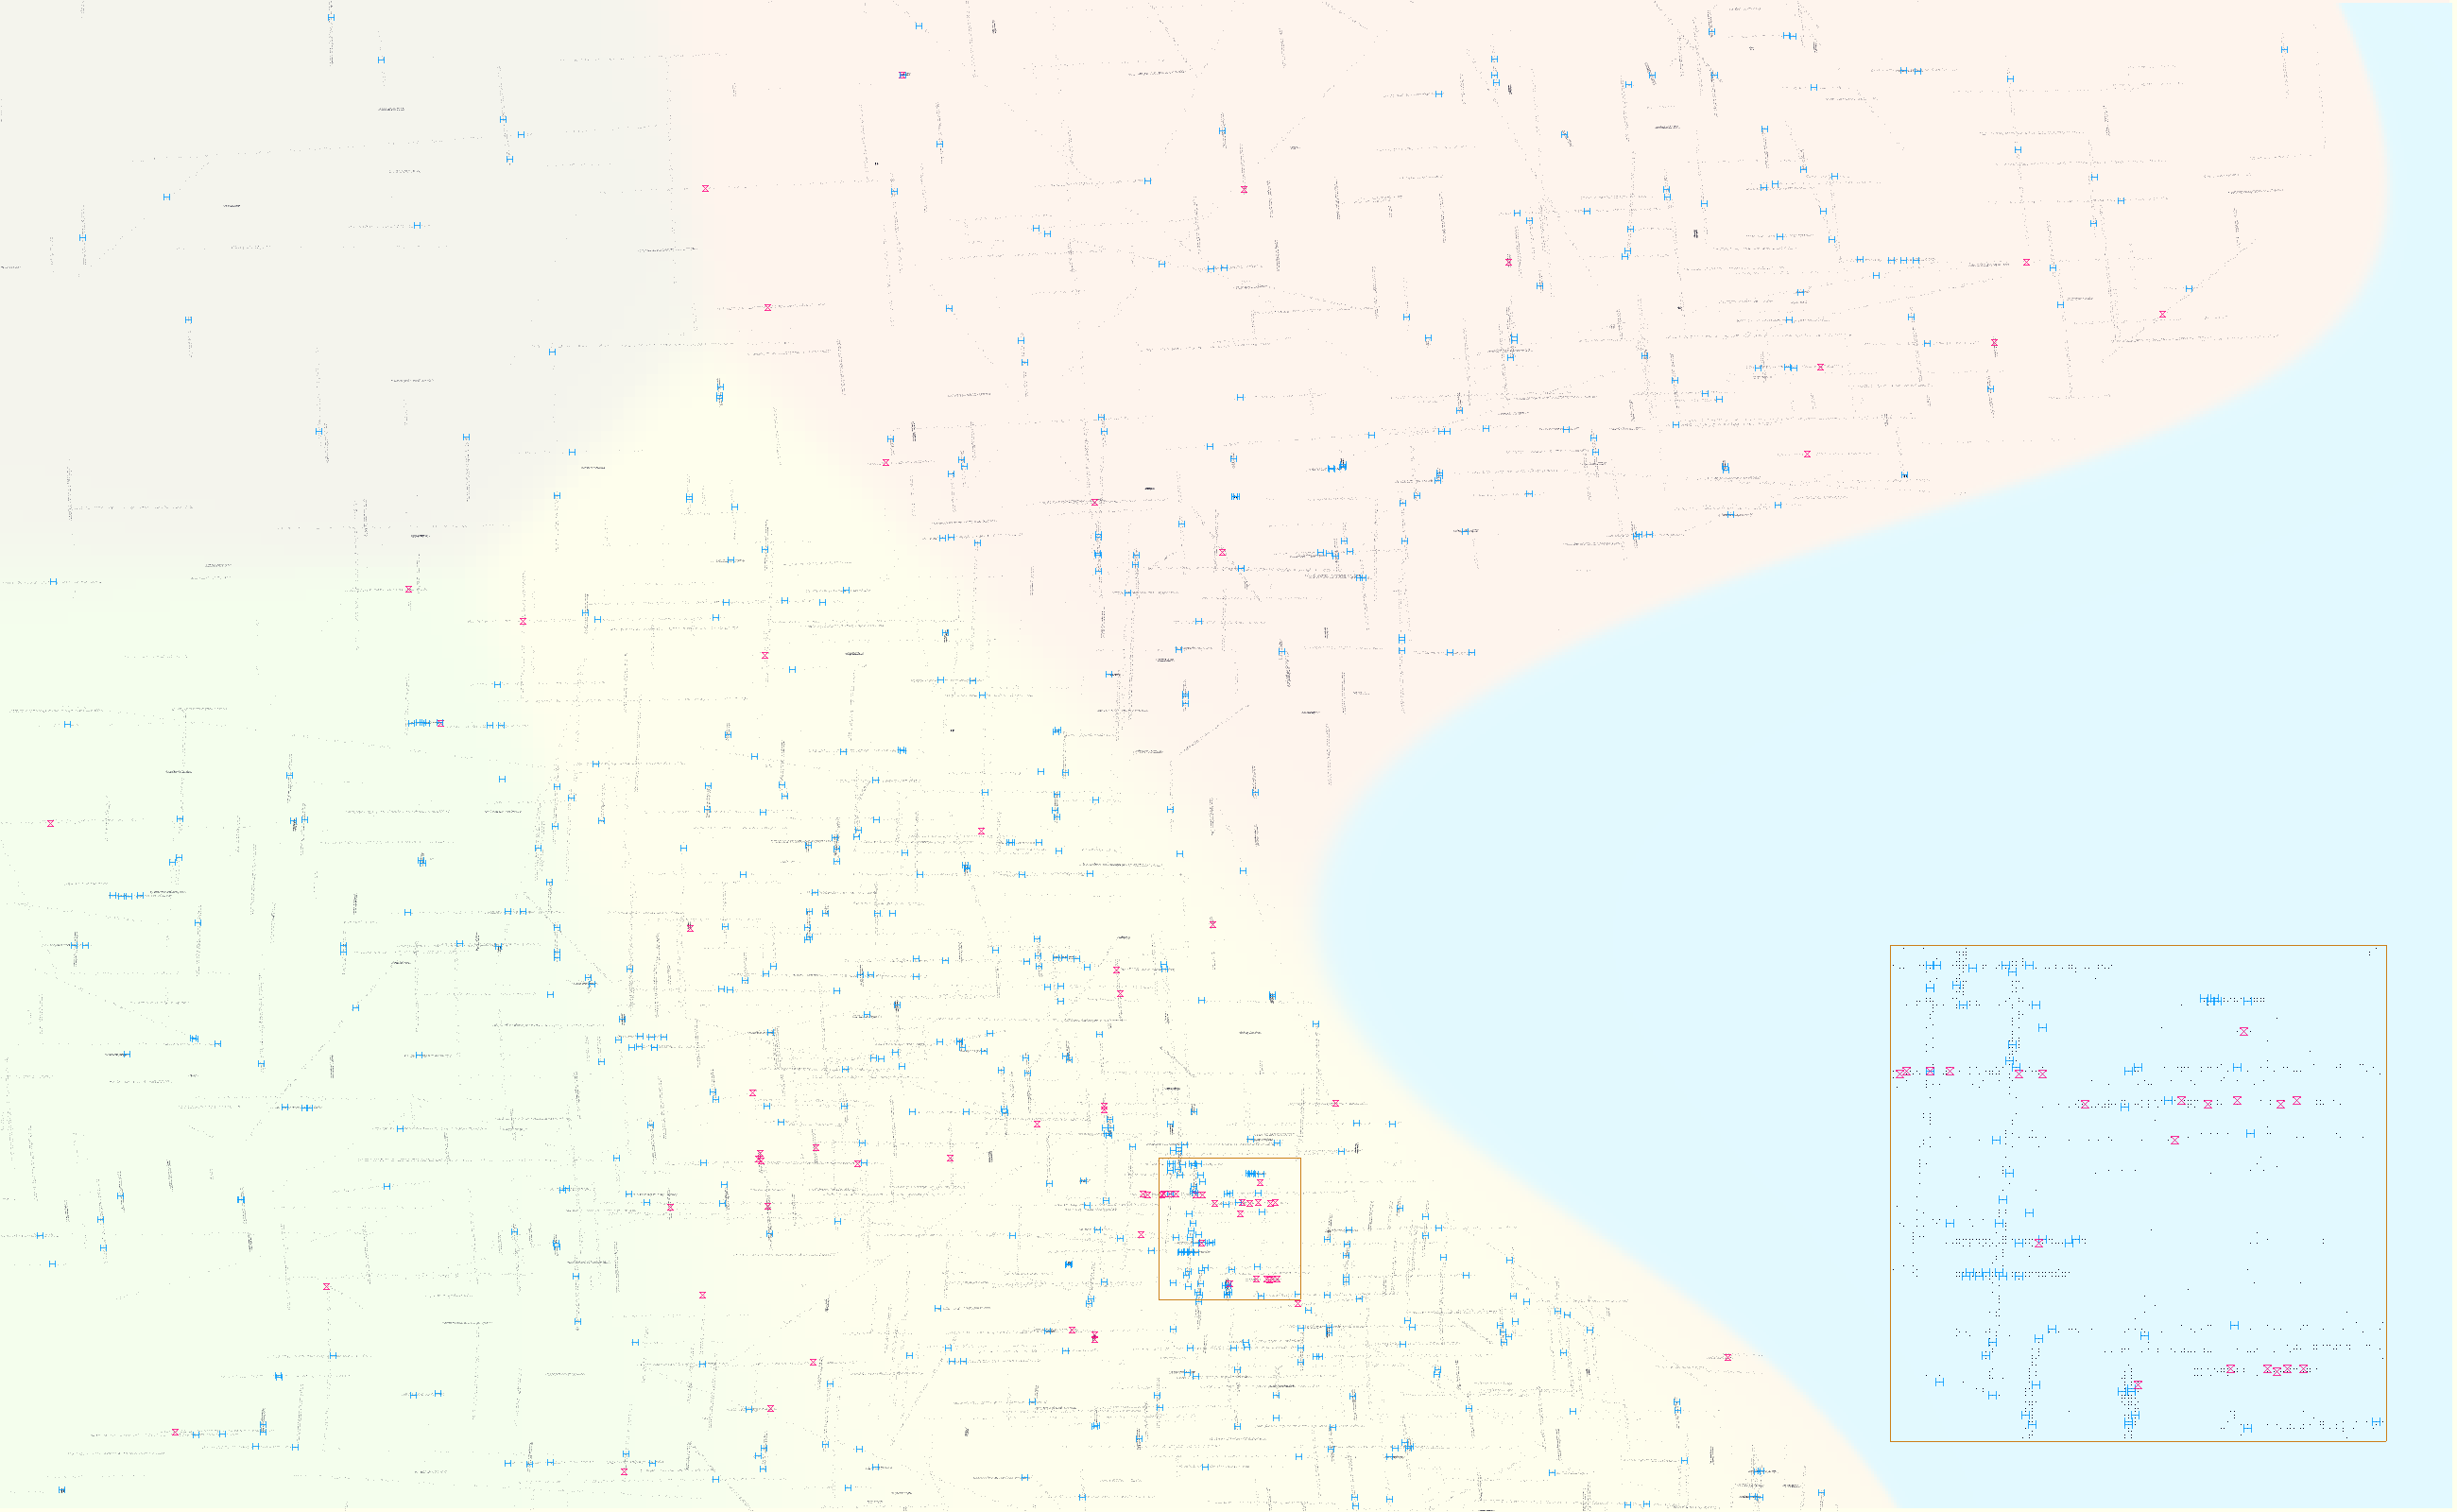
\includegraphics[width=\textwidth]{hei}
          \captionof{figure}{
            In light yellow and blue are land and sea: $6.4\text{km}\times
            10.4\text{km}$ around the city of Zembla.
            Gray dots:       untested faucets.
            Red bowties:     faucets tested positive.
            Blue I-beams:    faucets tested negative.
            The small yellow box surrounds a neighborhood that enjoyed more
            thorough testing; the large yellow box in the lower right magnifies
            that extra-tested region.
            %
            TODO: number of gray dots, among labels: training set vs hidden 
          }
        \end{figure}

      \pagebreak
        Cool! We see that the faucets (gray dots) are strongly concentrated
        along north-south and east-west line segments mostly $0.2\text{km}$ to
        $0.5\text{km}$ in length.  Do those segments reflect pipes aligned
        underground along roads?  Or perhaps they arose as an artifact, if
        these coordinates were inferred from city records of population density
        and of utility bills organized by street address?  Ideally we'd ask the
        city to clarify.  But let's say they ignored our emails; then we'll do
        an analysis agnostic to the exact interpretation of these segments.

        There seems to be some large-scale spatial dependence: contamination
        seems most prevalent in the bottom third of the map; it seems
        least prevalent in the middle third.
        Inspecting the zoomed section, we notice some small-scale spatial
        dependence, too: it seems plausible that faucet labels are highly
        correlated along each segment.

        Let's develop a simple model.  Each faucet $f$ belongs to a member
        $s(f)\in S$ of the set of segments.  Each faucet $f$ has scaled
        coordinates $\vec x(f) \in [-1,+1]^2$, and likewise for $\vec x(s)$ for
        the midpoint of segment $s$.
        $$
            p_s \sim \text{Beta}(q_{\vec x(s)}, 1-q_{\vec x(s)}) 
            \quad\quad
            \ell_f \sim \text{Bern}(p_{s(f)})
            %\ell_f \sim \text{Bern}(p_{s(f)} \text{~if~} c_f=1 \text{~else~} \sigma(q_{\vec x(f)}))
        $$
        Here, $q$ is some unknown function that tells us for each location
        $\vec x$ how likely a faucet near that location is contaminated.  We
        imagine $q$ as smoothly varying and as sampled from some
        translation-invariant distribution over functions.  It's thus natural
        to model $q$ as generated by a fourier series with random coefficients
        indexed by pairs $\vec k$ of integers:
        $$
            c_{\vec k} \sim \text{Gauss}(0,v_{\vec k}) + i\text{Gauss}(0,v_{\vec k})
            \quad\quad
            q_{\vec x} = \sigma \,\left[\, \mathfrak{Re} \, \sum_k c_{\vec k} \cdot \exp(\pi i {\vec k} \cdot {\vec x)} \, \right]
        $$
        A natural choice for the variances $v_{\vec k}$ is a power law like
        $v_{\vec k} = 1/(1+|k|)$; that's on the boundary of the energy
        diverging. This induces a brownian-motion-like Gaussian Process.

        %There is some probability distribution over configurations of segments.

        % nearest neighbor with p<1 non-norm (e.g. 1/2? or tuned?) to reflect axis alignment)
        %

      \samsubsubsection{featurization and fitting}
      \samsubsubsection{model selection}
      %\samsubsubsection{modeling and fitting}
      %\samsubsubsection{model selection}
      \samsubsubsection{prediction}
      \samsubsubsection{overfitting}

    \samsubsection{pairing flavors}
      \samsubsubsection{visualization}
      \samsubsubsection{modeling and fitting}
      \samsubsubsection{regularization}
      \samsubsubsection{explanation}
      \samsubsubsection{domain adaptation}

    \samsubsection{ancient tablets}
      \samsubsubsection{visualization}
      \samsubsubsection{transcription}
      \samsubsubsection{cleaning and imputation}
      \samsubsubsection{modeling and fitting}
      \samsubsubsection{generation}

  \samsection{statistics}
    \samsubsection{bayesian inference}%bayesian induction}
      \samquote{So little of what could happen does happen.}{salvador dali}



      \samsubsubsection{conceptual framework}
      We're confronted with an observation or dataset $\sfo$ that comes from
      some unknown underlying pattern $\sfh$.  We know how each possible value
      $h$ for $\sfh$ induces a distribution on $\sfo$ and we have a prior sense
      of which $h$s are probable.  Bayes' law helps us update this sense to
      account for the dataset by relating two functions of $h$:
      $$
        \underbrace{p_{\sfh|\sfo}(h|o)}_{\text{posterior}}
        \propto
        \underbrace{p_{\sfo|\sfh}(o|h)}_{\text{likelihood}}
        \cdot
        \underbrace{p_{\sfh}(h)}_{\text{prior}}
      $$

      Bayes' law underlies our analyses throughout these notes.
      %
      Like Newton's $F=ma$, Bayes is by itself inert: to make predictions we'd
      have to specify our situation's forces or likelihoods.  Continuing the
      metaphor, we will rarely solve our equations exactly; we'll instead make
      approximations good enough to build bridges and swingsets.  Still, no one
      denies that $F=ma$ orients us usefully in the world of physics.  So it is
      with the law of Bayes.

      %\samsubsubsection{formalism}
      Formally, we posit a set $\hH$ of \emph{hypotheses}, a set $\oO$ of
      possible \emph{observations}, and a set $\aA$ of permitted
      \emph{actions}.  We assume as given a joint probability measure
      $p_{\sfo,\sfh}$ on $\oO\times \hH$ and a \emph{cost function}
      $c:\aA\times \hH \to \Rr$.
      %
      That cost function says how much it hurts to take the action $a\in \aA$
      when the truth is $h\in \hH$.
      %
      Our primary aim is to construct a map $\pi:\oO\to \aA$ that makes the
      expected cost $\Ee_{\sfh,\sfo} \, c(\pi(\sfa); \sfh)$ small.

      Below are three examples.  In each case, we're designing a robotic vacuum
      cleaner: $\hH$ contains possible floor plans; $\oO$, 
      possible readings from the robot's sensors.  The examples differ in how
      they define and interpret $\aA$ and $c$.

      \textbf{A}.  $\aA$ consists of probability distributions over $\hH$. We
      regard $\pi(o)$ as giving a posterior distribution on $\hH$ upon
      observation $o$.  Our cost $c(a;h)$ measures the surprise of someone who
      believes $a$ upon learning that $h$ is true. 
      %
      Such \emph{inference problems}, being in a precise sense universal, pose
      huge computational difficulties; we thus often collapse distributions to
      points, giving rise to the distinctive challenge of balancing estimation
      error with structural error.

      \textbf{B}.
      $\aA$ consists of latitude-longitude pairs, interpreted as a guessed
      location of the robot's charging station.  The cost $c(a;h)$ measures how
      distant our guess is from the truth.  
      %
      Such \emph{estimation problems} abound in science and engineering; they
      pose the distinctive challenge of balancing
      sensitivity-to-misleading-outliers against
      sensitivity-to-informative-datapoints.
      %robustness to measurement noise with
      %centeredness. 

      \textbf{C}.  $\aA$ consists of instructions we may send to the motors,
      instructions that induce motion through our partially-known room.  The
      cost $c(a;h)$ incentivizes motion into dusty spaces and penalizes bumping
      into walls.
      %
      We often compose such \emph{decision problems} sequentially; this gives
      rise to the distinctive challenge of balancing exploration with
      exploitation.

      \samsubsubsection{frequentism and choice of prior}
      %\samquote{
      %  I am wiser [than he] ... for
      %  ... he fancies he knows something 
      %  ... whereas I ... do not fancy I do.
      %}{socrates}
      %\samsubsubsection{uniform priors} % jeffries
        Our engineering culture prizes not just \emph{utility} but also
        \emph{confidence}, since strong guarantees on our designs allow 
        composition of our work into larger systems: equality, unlike
        similarity, is transitive.  For example, we'd often prefer a 99\%
        guarantee of adequate performance over a 90\% guarantee of ideal
        performance.  This asymmetry explains our pessimistic obsession with
        worst-case bounds over best-case bounds, cost functions over fitness
        functions, and simple models with moderate-but-estimatable errors over
        rich models with unknownable-but-often-small errors.

        The \emph{frequentist} or \emph{distribution-free} style of statistics
        continues this risk-averse tradition.  In the fullest instance of this
        style, we do inference as if the true unknown prior on $\hH$ is chosen
        adversarially.
        %
        That is, we try to find $\pi$ that makes the following error small:
        $$
          \max_{p_{\sfh}}
          \,
          \Ee_{\sfh \sim p_{\sfh}(\cdot)} \Ee_{\sfo \sim p_{\sfo}(\cdot|\sfh)}
          \,
          c(\pi(\sfo); \sfh) 
        $$
        %
        %For example, suppose $\aA=\hH$ and $c(a;h) = [\![a\neq h]\!]$ is the
        %zero-one cost.
        %The prior in the minimax pair $(\pi, p_{\sfh})$ tends to be pretty
        %uniform. 
        Intuitively, 

        %minimax 
        %``uniform'' prior
        %on hypothesis space.

      \samsubsubsection{p-hacking} % likelihoods, confidence intervals 
      \samsubsubsection{hidden assumptions} % distribution-existence as coherence condition

    \samsubsection{(multiple) hypothesis testing}
      %\samquote{
      %  The theory of probabilities is at bottom nothing but common sense
      %  reduced to calculus; it enables us to appreciate with exactness
      %  [what we] feel with a sort of instinct ...
      %}{pierre simon laplace}

      Let's now consider the case where $\hH$ is a small and finite.  We

    \samsubsection{covariance, correlation, least squares}
      
    \samsubsection{gradient descent}
      \samquote{
        The key to success is failure.
      }{michael j.\ jordan}

      In what follows, 
        \texttt{init} returns a point in $\pP$,
        \texttt{rate} is a small positive real number,
        \texttt{time} is a large natural number, and
        \texttt{loss} is a function $:\pP\to\Rr$ amenable to differentiation. 
      An important hidden input to gradient descent is the choice of transpose
      function; this function converts row vectors to column vectors and thus
      biases learning just as a choice of svm kernel does.
      \begin{lstlisting}[language=Python, mathescape=true, basicstyle=\ttfamily]
        def gd(init, rate, time, loss):
          $\theta$ = init()
          for t in range(time):
            $\theta$ -= rate * ($\nabla$loss($\theta$))$^\text{transpose}$ 
          return $\theta$
      \end{lstlisting}

      \samsubsubsection{smoothness}
      \samsubsubsection{deep learning}
      \samsubsubsection{optimizers} % critical points, local vs global minima, momentum, etc 
      \samsubsubsection{initialization} % expectation maximization 
      \samsubsubsection{expectation maximization}

  \samsection{high dimensions}
    \samsubsection{what is it like to live in high dimensions?}
      \samsubsubsection{weird balls}
      \samsubsubsection{concentration}
      \samsubsubsection{sparsity, rank, submanifolds}
      \samsubsubsection{visualization}

    \samsubsection{classification and clustering}
      \samquote{It is written that animals are divided into (a) those
        belonging to the emperor; (b) embalmed ones; (c) trained ones; (d)
        suckling pigs; (e) mermaids; (f) fabled ones; (g) stray dogs; (h) those
        included in this classification; (i) those that tremble as if they were
        mad; (j) innumerable ones; (k) those drawn with a very fine camel hair
        brush; (l) et cetera; (m) those that have just broken the vase; and (n)
        those that from afar look like flies.}{jorge luis borges}

    \samsubsection{graphical models}
      \samquote{
        ... [to treat] complicated systems in simple ways[,] probability ...
        implements two principles[:] [the approximation of parts as
        independent] and [the abstraction of aspects as their averages].
      }{michael i. jordan}


    \samsubsection{tool of the trade: boosted trees} %\samsubsection{ensembles}
      \samquote{
        Doing ensembles and shows is one thing, but being able to front a
        feature is totally different.  ...  there's something about ... a
        feature that's unique. 
      }{michael b.\ jordan}

  \samsection{networks}
  \samsection{time series}
  \samsection{gaussian processes}

  \samsection{appendix}%: background}
    \samsubsection{notation and math refresher}
      \samsubsubsection{probability and matrix notation}
        We've tried to use 
          \vspace{-0.10cm}
        $$
          \text{\textsf{sans serif} for the names of random variables,}
          \vspace{-0.15cm}
        $$
        $$
          \text{\emph{italics} for the values they may take, and}
        $$
        $$
          \text{$\mathcal{CURLY~CAPS}$ for sets of such values.} 
        $$
        For example, we write $p_{\sfy|\sfh}(y|h)$ for the probability that the
        random variable $\sfy$ takes the value $y$ conditioned on the event that
        the random variable $\sfh$ takes the value $h$.
        %
        Likewise, our notation $p_{\hat \sfh|\sfh}(h|h)$ indicates the
        probability that the random variables $\hat \sfh$ and $\sfh$ agree in
        value given that $\sfh$ takes a value $h\in \hH$.


      \samsubsubsection{probability}
      \samsubsubsection{linear algebra}
      \samsubsubsection{calculus}
      \samsubsubsection{concentration}

    \samsubsection{python programming refresher}
      \samsubsubsection{setup}
      \samsubsubsection{state and control flow}
      \samsubsubsection{input/output}
      \samsubsubsection{numpy}

  %\samsection{appendix: bonus topics}
    \samsubsection{beyond the i.i.d.\ hypothesis}
      \samsubsubsection{out-of-distribution tests}
      \samsubsubsection{dependent samples}
      \samsubsubsection{causality}
    %\samsubsection{representation learning}
    %\samsubsection{recommended reading}


\end{document}



